\documentclass{agony}
\title{SPH4U: Dynamics Assignment}

\begin{document}
\thispagestyle{firstpage}
\textbf{\thetitle}

\begin{prob}
	\phantom{}
	\begin{enumerate}[(a)]
		\item \textbf{Draw FBD(s).}\\
		      \begin{minipage}[t]{.5\textwidth}
			      \underline{$m_{1}$ FBD:}
			      \tikzset{every picture/.style={line width=0.75pt}} %set default line width to 0.75pt        

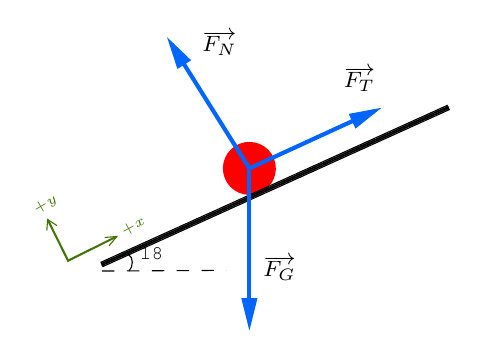
\begin{tikzpicture}[x=0.75pt,y=0.75pt,yscale=-1,xscale=1]
	%uncomment if require: \path (0,300); %set diagram left start at 0, and has height of 300

	%Shape: Ellipse [id:dp1428949648769431] 
	\draw  [color={rgb, 255:red, 255; green, 0; blue, 0 }  ,draw opacity=1 ][fill={rgb, 255:red, 254; green, 0; blue, 0 }  ,fill opacity=1 ] (149.04,183.11) .. controls (147.8,176.33) and (152.3,169.83) .. (159.09,168.59) .. controls (165.87,167.35) and (172.38,171.85) .. (173.61,178.64) .. controls (174.85,185.42) and (170.35,191.93) .. (163.56,193.16) .. controls (156.78,194.4) and (150.28,189.9) .. (149.04,183.11) -- cycle ;
	%Shape: Rectangle [id:dp48287918810377195] 
	\draw   (89.84,226.09) -- (256.64,150.53) -- (256.96,151.22) -- (90.15,226.78) -- cycle ;
	%Shape: Rectangle [id:dp005233673921997584] 
	\draw   (90.15,226.78) -- (256.96,151.22) -- (257.27,151.91) -- (90.46,227.47) -- cycle ;
	%Shape: Rectangle [id:dp9526931686132831] 
	\draw   (90.46,227.47) -- (257.27,151.91) -- (257.58,152.6) -- (90.77,228.16) -- cycle ;

	%Straight Lines [id:da8350690671631047] 
	\draw [color={rgb, 255:red, 1; green, 101; blue, 255 }  ,draw opacity=1 ][line width=1.5]    (161.33,180.88) -- (161.33,255.01) ;
	\draw [shift={(161.33,259.01)}, rotate = 270] [fill={rgb, 255:red, 1; green, 101; blue, 255 }  ,fill opacity=1 ][line width=0.08]  [draw opacity=0] (15.6,-3.9) -- (0,0) -- (15.6,3.9) -- cycle    ;
	%Straight Lines [id:da1062981577052522] 
	\draw [color={rgb, 255:red, 1; green, 101; blue, 255 }  ,draw opacity=1 ][line width=1.5]    (161.33,180.88) -- (123.79,121.05) ;
	\draw [shift={(121.67,117.67)}, rotate = 57.89] [fill={rgb, 255:red, 1; green, 101; blue, 255 }  ,fill opacity=1 ][line width=0.08]  [draw opacity=0] (15.6,-3.9) -- (0,0) -- (15.6,3.9) -- cycle    ;
	%Straight Lines [id:da21972886949175963] 
	\draw [color={rgb, 255:red, 1; green, 101; blue, 255 }  ,draw opacity=1 ][line width=1.5]    (161.33,180.88) -- (221.36,153.33) ;
	\draw [shift={(225,151.67)}, rotate = 155.36] [fill={rgb, 255:red, 1; green, 101; blue, 255 }  ,fill opacity=1 ][line width=0.08]  [draw opacity=0] (15.6,-3.9) -- (0,0) -- (15.6,3.9) -- cycle    ;
	%Shape: Right Angle [id:dp7929492774408056] 
	\draw  [color={rgb, 255:red, 65; green, 117; blue, 5 }  ,draw opacity=1 ][line width=0.75]  (97.31,213.73) -- (73.99,225.35) -- (64.15,205.57) ;
	\draw  [color={rgb, 255:red, 65; green, 117; blue, 5 }  ,draw opacity=1 ] (63.75,210.84) -- (64.11,205.52) -- (68.6,208.42) ;
	\draw  [color={rgb, 255:red, 65; green, 117; blue, 5 }  ,draw opacity=1 ] (91.56,214.16) -- (97.45,213.7) -- (93.7,218.23) ;

	%Curve Lines [id:da5437896212575373] 
	\draw    (103,222.33) .. controls (105.67,223.67) and (105.33,228.33) .. (103.33,230.33) ;
	%Straight Lines [id:da9621621519167294] 
	\draw  [dash pattern={on 4.5pt off 4.5pt}]  (90.33,230.33) -- (150.33,230) ;

	% Text Node
	\draw (166.85,221.91) node [anchor=north west][inner sep=0.75pt]  [font=\footnotesize] [align=left] {$\displaystyle \overrightarrow{F_{G}}$};
	% Text Node
	\draw (205.56,130.62) node [anchor=north west][inner sep=0.75pt]  [font=\footnotesize] [align=left] {$\displaystyle \overrightarrow{F_{T}}$};
	% Text Node
	\draw (137.43,113.35) node [anchor=north west][inner sep=0.75pt]  [font=\footnotesize,color={rgb, 255:red, 0; green, 0; blue, 0 }  ,opacity=1 ] [align=left] {$\displaystyle \overrightarrow{F_{N}}$};
	% Text Node
	\draw (107.33,218) node [anchor=north west][inner sep=0.75pt]  [font=\scriptsize] [align=left] {{\fontfamily{pcr}\selectfont 18}$\displaystyle \degree $};
	% Text Node
	\draw (97.11,208.66) node [anchor=north west][inner sep=0.75pt]  [font=\tiny,color={rgb, 255:red, 65; green, 117; blue, 5 }  ,opacity=1 ,rotate=-331] [align=left] {$\displaystyle +x$};
	% Text Node
	\draw (54.78,198.23) node [anchor=north west][inner sep=0.75pt]  [font=\tiny,color={rgb, 255:red, 65; green, 117; blue, 5 }  ,opacity=1 ,rotate=-329.58] [align=left] {$\displaystyle +y$};


\end{tikzpicture}
		      \end{minipage}%
		      \begin{minipage}[t]{.5\textwidth}
			      \underline{$m_{2}$ FBD:}
			      

\tikzset{every picture/.style={line width=0.75pt}} %set default line width to 0.75pt        

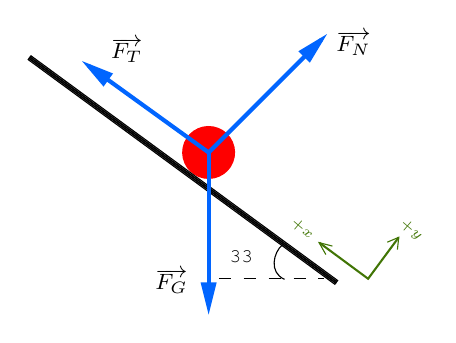
\begin{tikzpicture}[x=0.75pt,y=0.75pt,yscale=-1,xscale=1]
	%uncomment if require: \path (0,300); %set diagram left start at 0, and has height of 300

	%Shape: Ellipse [id:dp1428949648769431] 
	\draw  [color={rgb, 255:red, 255; green, 0; blue, 0 }  ,draw opacity=1 ][fill={rgb, 255:red, 254; green, 0; blue, 0 }  ,fill opacity=1 ] (198.05,181.45) .. controls (199.28,174.66) and (194.78,168.16) .. (188,166.92) .. controls (181.21,165.69) and (174.71,170.19) .. (173.47,176.97) .. controls (172.24,183.76) and (176.74,190.26) .. (183.52,191.5) .. controls (190.31,192.73) and (196.81,188.23) .. (198.05,181.45) -- cycle ;
	%Shape: Rectangle [id:dp48287918810377195] 
	\draw   (247.91,240.87) -- (100.19,132.64) -- (99.74,133.25) -- (247.46,241.49) -- cycle ;
	%Shape: Rectangle [id:dp005233673921997584] 
	\draw   (247.46,241.49) -- (99.74,133.25) -- (99.29,133.87) -- (247.01,242.1) -- cycle ;
	%Shape: Rectangle [id:dp9526931686132831] 
	\draw   (247.01,242.1) -- (99.29,133.87) -- (98.85,134.48) -- (246.56,242.71) -- cycle ;

	%Straight Lines [id:da8350690671631047] 
	\draw [color={rgb, 255:red, 1; green, 101; blue, 255 }  ,draw opacity=1 ][line width=1.5]    (185.76,179.21) -- (185.76,253.35) ;
	\draw [shift={(185.76,257.35)}, rotate = 270] [fill={rgb, 255:red, 1; green, 101; blue, 255 }  ,fill opacity=1 ][line width=0.08]  [draw opacity=0] (15.6,-3.9) -- (0,0) -- (15.6,3.9) -- cycle    ;
	%Straight Lines [id:da1062981577052522] 
	\draw [color={rgb, 255:red, 1; green, 101; blue, 255 }  ,draw opacity=1 ][line width=1.5]    (185.76,179.21) -- (239.99,124.98) ;
	\draw [shift={(242.82,122.15)}, rotate = 135] [fill={rgb, 255:red, 1; green, 101; blue, 255 }  ,fill opacity=1 ][line width=0.08]  [draw opacity=0] (15.6,-3.9) -- (0,0) -- (15.6,3.9) -- cycle    ;
	%Straight Lines [id:da21972886949175963] 
	\draw [color={rgb, 255:red, 1; green, 101; blue, 255 }  ,draw opacity=1 ][line width=1.5]    (185.76,179.21) -- (128.01,137.53) ;
	\draw [shift={(124.77,135.19)}, rotate = 35.82] [fill={rgb, 255:red, 1; green, 101; blue, 255 }  ,fill opacity=1 ][line width=0.08]  [draw opacity=0] (15.6,-3.9) -- (0,0) -- (15.6,3.9) -- cycle    ;
	%Shape: Right Angle [id:dp7929492774408056] 
	\draw  [color={rgb, 255:red, 65; green, 117; blue, 5 }  ,draw opacity=1 ][line width=0.75]  (239.14,222.71) -- (262.61,240.05) -- (277.31,220.15) ;
	\draw  [color={rgb, 255:red, 65; green, 117; blue, 5 }  ,draw opacity=1 ] (276.72,226.04) -- (277.35,220.09) -- (271.84,222.43) ;
	\draw  [color={rgb, 255:red, 65; green, 117; blue, 5 }  ,draw opacity=1 ] (245.39,224.3) -- (238.99,222.65) -- (242.24,228.38) ;

	%Curve Lines [id:da5437896212575373] 
	\draw    (221.33,223.67) .. controls (217,227.33) and (214.67,237) .. (222.33,240.33) ;
	%Straight Lines [id:da5100408990791785] 
	\draw  [dash pattern={on 4.5pt off 4.5pt}]  (190.67,240) -- (241.33,240) ;

	% Text Node
	\draw (158.85,233.91) node [anchor=north west][inner sep=0.75pt]  [font=\footnotesize] [align=left] {$\displaystyle \overrightarrow{F_{G}}$};
	% Text Node
	\draw (137.56,122.62) node [anchor=north west][inner sep=0.75pt]  [font=\footnotesize] [align=left] {$\displaystyle \overrightarrow{F_{T}}$};
	% Text Node
	\draw (246.09,119.35) node [anchor=north west][inner sep=0.75pt]  [font=\footnotesize,color={rgb, 255:red, 0; green, 0; blue, 0 }  ,opacity=1 ] [align=left] {$\displaystyle \overrightarrow{F_{N}}$};
	% Text Node
	\draw (194.67,225) node [anchor=north west][inner sep=0.75pt]  [font=\scriptsize] [align=left] {{\fontfamily{pcr}\selectfont 33}$\displaystyle \degree $};
	% Text Node
	\draw (227.99,208.32) node [anchor=north west][inner sep=0.75pt]  [font=\tiny,color={rgb, 255:red, 65; green, 117; blue, 5 }  ,opacity=1 ,rotate=-40.39] [align=left] {$\displaystyle +x$};
	% Text Node
	\draw (280.67,208.71) node [anchor=north west][inner sep=0.75pt]  [font=\tiny,color={rgb, 255:red, 65; green, 117; blue, 5 }  ,opacity=1 ,rotate=-40.39] [align=left] {$\displaystyle +y$};


\end{tikzpicture}
		      \end{minipage}

		\item \textbf{Find the magnitude of the tension in the cable.}\\
		      \underline{$m_{1}$:}
		      \begin{solution}
			      \vec{F_{net_{1x}}}            & = 0                                                              \\
			      0                             & = \left\lvert\vec{F_{T}}\right\rvert - \vec{F_{g_{x}}}  \\
			      0                             & = \left\lvert\vec{F_{T}}\right\rvert - 380(9.81) \sin 18 \degree      \\
			      \left\lvert\vec{F_{T}}\right\rvert & = 380(9.81) \sin 18 \degree \\
			      \left\lvert\vec{F_{T}}\right\rvert & = 1151.95~\text{N}\\
			      \left\lvert\vec{F_{T}}\right\rvert & = 1200~\text{N}
		      \end{solution}
		      \framebox{$\therefore$ The magnitude of tension in the cable is \textbf{1200 N}.}

		\item \textbf{Calculate the mass of \bm{$m_{2}$} needed to keep the system in equilibrium.}

		      \begin{solution}
			      \vec{F_{net_{2x}}} & = 0\\
			      0 &= \vec{F_{T}} - \vec{F_{g_{x}}}\\
			      0 &= 1151.95 - m_{2}(9.81)\sin33\degree\\
			      m_{2} &= \frac{1151.95}{9.81\sin33\degree}\\
			      m_{2} &= 215.6~\text{kg}\\
			      m_{2} &= 220~\text{kg}
		      \end{solution}
		      \framebox{$\therefore$ The mass of the second box ($m_{2}$) is \textbf{220 kg}.}
	\end{enumerate}
\end{prob}

\begin{prob}
	\phantom{}
	\begin{enumerate}[(a)]
		\item \textbf{What will be the horizontal acceleration of the bale?}\\
		      \begin{minipage}{0.3\textwidth}
			      \tikzset{every picture/.style={line width=0.75pt}} %set default line width to 0.75pt        

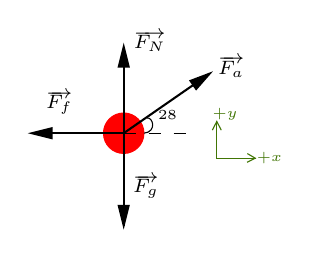
\begin{tikzpicture}[x=0.75pt,y=0.75pt,yscale=-1,xscale=1]
	%uncomment if require: \path (0,300); %set diagram left start at 0, and has height of 300

	%Shape: Ellipse [id:dp7093999861642637] 
	\draw  [color={rgb, 255:red, 255; green, 0; blue, 0 }  ,draw opacity=1 ][fill={rgb, 255:red, 255; green, 0; blue, 0 }  ,fill opacity=1 ] (186.23,101.02) .. controls (186.23,95.64) and (190.58,91.29) .. (195.96,91.29) .. controls (201.33,91.29) and (205.69,95.64) .. (205.69,101.02) .. controls (205.69,106.39) and (201.33,110.75) .. (195.96,110.75) .. controls (190.58,110.75) and (186.23,106.39) .. (186.23,101.02) -- cycle ;
	%Straight Lines [id:da6548156036946866] 
	\draw [line width=0.75]    (195.96,101.02) -- (195.96,59.41) ;
	\draw [shift={(195.96,57.41)}, rotate = 90] [fill={rgb, 255:red, 0; green, 0; blue, 0 }  ][line width=0.08]  [draw opacity=0] (12,-3) -- (0,0) -- (12,3) -- cycle    ;
	%Straight Lines [id:da7473835217170912] 
	\draw [line width=0.75]    (195.96,101.02) -- (237.34,72.33) ;
	\draw [shift={(238.98,71.19)}, rotate = 145.27] [fill={rgb, 255:red, 0; green, 0; blue, 0 }  ][line width=0.08]  [draw opacity=0] (12,-3) -- (0,0) -- (12,3) -- cycle    ;
	%Straight Lines [id:da852905721719166] 
	\draw [line width=0.75]    (195.96,101.02) -- (151.75,101.02) ;
	\draw [shift={(149.75,101.02)}, rotate = 360] [fill={rgb, 255:red, 0; green, 0; blue, 0 }  ][line width=0.08]  [draw opacity=0] (12,-3) -- (0,0) -- (12,3) -- cycle    ;
	%Straight Lines [id:da7879707425395328] 
	\draw [line width=0.75]    (195.96,101.02) -- (195.96,145.5) ;
	\draw [shift={(195.96,147.5)}, rotate = 270] [fill={rgb, 255:red, 0; green, 0; blue, 0 }  ][line width=0.08]  [draw opacity=0] (12,-3) -- (0,0) -- (12,3) -- cycle    ;
	%Shape: Right Angle [id:dp015604455251778004] 
	\draw  [color={rgb, 255:red, 65; green, 117; blue, 5 }  ,draw opacity=1 ] (259.53,113.15) -- (240.84,113.15) -- (240.84,95.32) ;
	\draw  [color={rgb, 255:red, 65; green, 117; blue, 5 }  ,draw opacity=1 ] (242.96,99.54) -- (240.81,95.35) -- (238.68,99.55) ;
	\draw  [color={rgb, 255:red, 65; green, 117; blue, 5 }  ,draw opacity=1 ] (255.4,115.02) -- (259.34,113.06) -- (255.53,110.83) ;

	%Curve Lines [id:da9919868327074761] 
	\draw    (205.69,101.02) .. controls (212.28,100.3) and (209.87,92.89) .. (207.11,93.76) ;
	%Straight Lines [id:da6820111378004245] 
	\draw  [dash pattern={on 4.5pt off 4.5pt}]  (195.96,101.02) -- (225.89,101.02) ;

	% Text Node
	\draw (199.61,50.44) node [anchor=north west][inner sep=0.75pt]  [font=\scriptsize] [align=left] {$\displaystyle \overrightarrow{F_{N}}$};
	% Text Node
	\draw (240.22,62.76) node [anchor=north west][inner sep=0.75pt]  [font=\scriptsize] [align=left] {$\displaystyle \overrightarrow{F_{a}}$};
	% Text Node
	\draw (157.27,79.34) node [anchor=north west][inner sep=0.75pt]  [font=\scriptsize] [align=left] {$\displaystyle \overrightarrow{F_{f}}$};
	% Text Node
	\draw (199.25,119.91) node [anchor=north west][inner sep=0.75pt]  [font=\scriptsize] [align=left] {$\displaystyle \overrightarrow{F_{g}}$};
	% Text Node
	\draw (211.24,88.8) node [anchor=north west][inner sep=0.75pt]  [font=\tiny] [align=left] {$\displaystyle 28\degree $};
	% Text Node
	\draw (258.87,108.89) node [anchor=north west][inner sep=0.75pt]  [font=\tiny,color={rgb, 255:red, 65; green, 117; blue, 5 }  ,opacity=1 ] [align=left] {$\displaystyle +x$};
	% Text Node
	\draw (237.51,87.53) node [anchor=north west][inner sep=0.75pt]  [font=\tiny,color={rgb, 255:red, 65; green, 117; blue, 5 }  ,opacity=1 ] [align=left] {$\displaystyle +y$};


\end{tikzpicture}
		      \end{minipage}%
		      \begin{minipage}{0.3\textwidth}
			      \vspace{-8mm}
			      \begin{flalign*}
				      \vec{F_{net_{x}}} & = \vec{F_{a_{x}}} - \vec{F_{f}}   \\
				                        & = 140 \cos 28\degree - 55         \\
				                        & = 68.81~\text{N[forward]}       &
			      \end{flalign*}
		      \end{minipage}%
		      \begin{minipage}{0.3\textwidth}
			      \vspace{-8mm}
			      \begin{flalign*}
				      \vec{F_{net_{x}}} & = m\vec{a}                                     \\
				      68.81             & = 35\vec{a}                                    \\
				      \vec{a}           & = 1.96\text{m/s\textsuperscript{2}[forward]}   \\
				      \vec{a}           & = 2.0~\text{m/s\textsuperscript{2}[forward]} &
			      \end{flalign*}
		      \end{minipage}%
		      \vspace{2mm}
		      \\\framebox{$\therefore$ The horizontal acceleration of the bale will be \textbf{2.0 m/s\textsuperscript{2}[forward].}}
		      \newpage
		\item \textbf{What is the coefficient of friction between the bale and the ground?}
		      \begin{solution}
			      \vec{F_{f}} &= \mu_{f}\vec{F_{N}}\\
			      55 &= \mu_{f}(\vec{F_{g}} - \vec{F_{a_{y}}})\\
			      \mu_{f} &= \frac{55}{\vec{F_{g}} - \vec{F_{a_{y}}}}\\
			      \mu_{f} &= \frac{55}{35(9.81)-140\sin 28\degree}\\
			      \mu_{f} &= 0.198\\
			      \mu_{f} &= 0.20
		      \end{solution}
		      \framebox{$\therefore$ The coefficient of friction between the bale and ground is \textbf{0.20}.}
	\end{enumerate}

\end{prob}

\begin{prob}
	\phantom{}
	\begin{enumerate}[(a)]
		\item \textbf{Draw an FBD showing a tilted coordinate system (label positive x-direction)}\\
		      \begin{center}
			      \tikzset{every picture/.style={line width=0.75pt}} %set default line width to 0.75pt        

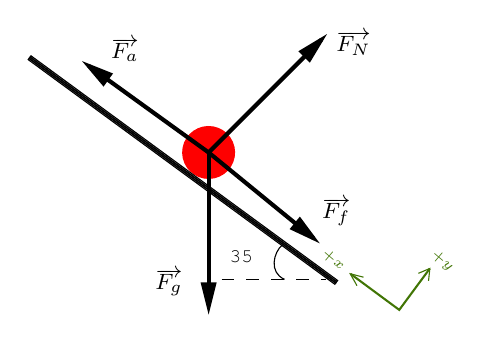
\begin{tikzpicture}[x=0.75pt,y=0.75pt,yscale=-1,xscale=1]
	%uncomment if require: \path (0,300); %set diagram left start at 0, and has height of 300

	%Shape: Ellipse [id:dp1428949648769431] 
	\draw  [color={rgb, 255:red, 255; green, 0; blue, 0 }  ,draw opacity=1 ][fill={rgb, 255:red, 254; green, 0; blue, 0 }  ,fill opacity=1 ] (198.05,181.45) .. controls (199.28,174.66) and (194.78,168.16) .. (188,166.92) .. controls (181.21,165.69) and (174.71,170.19) .. (173.47,176.97) .. controls (172.24,183.76) and (176.74,190.26) .. (183.52,191.5) .. controls (190.31,192.73) and (196.81,188.23) .. (198.05,181.45) -- cycle ;
	%Shape: Rectangle [id:dp48287918810377195] 
	\draw   (247.91,240.87) -- (100.19,132.64) -- (99.74,133.25) -- (247.46,241.49) -- cycle ;
	%Shape: Rectangle [id:dp005233673921997584] 
	\draw   (247.46,241.49) -- (99.74,133.25) -- (99.29,133.87) -- (247.01,242.1) -- cycle ;
	%Shape: Rectangle [id:dp9526931686132831] 
	\draw   (247.01,242.1) -- (99.29,133.87) -- (98.85,134.48) -- (246.56,242.71) -- cycle ;

	%Straight Lines [id:da8350690671631047] 
	\draw [color={rgb, 255:red, 0; green, 0; blue, 0 }  ,draw opacity=1 ][line width=1.5]    (185.76,179.21) -- (185.76,253.35) ;
	\draw [shift={(185.76,257.35)}, rotate = 270] [fill={rgb, 255:red, 0; green, 0; blue, 0 }  ,fill opacity=1 ][line width=0.08]  [draw opacity=0] (15.6,-3.9) -- (0,0) -- (15.6,3.9) -- cycle    ;
	%Straight Lines [id:da1062981577052522] 
	\draw [color={rgb, 255:red, 0; green, 0; blue, 0 }  ,draw opacity=1 ][line width=1.5]    (185.76,179.21) -- (239.99,124.98) ;
	\draw [shift={(242.82,122.15)}, rotate = 135] [fill={rgb, 255:red, 0; green, 0; blue, 0 }  ,fill opacity=1 ][line width=0.08]  [draw opacity=0] (15.6,-3.9) -- (0,0) -- (15.6,3.9) -- cycle    ;
	%Straight Lines [id:da21972886949175963] 
	\draw [color={rgb, 255:red, 0; green, 0; blue, 0 }  ,draw opacity=1 ][line width=1.5]    (185.76,179.21) -- (128.01,137.53) ;
	\draw [shift={(124.77,135.19)}, rotate = 35.82] [fill={rgb, 255:red, 0; green, 0; blue, 0 }  ,fill opacity=1 ][line width=0.08]  [draw opacity=0] (15.6,-3.9) -- (0,0) -- (15.6,3.9) -- cycle    ;
	%Shape: Right Angle [id:dp7929492774408056] 
	% \draw  [color={rgb, 255:red, 65; green, 117; blue, 5 }  ,draw opacity=1 ][line width=0.75]  (281.02,261.19) -- (255.11,241.93) -- (271.45,219.97) ;
	% \draw  [color={rgb, 255:red, 65; green, 117; blue, 5 }  ,draw opacity=1 ] (265.4,222.48) -- (271.49,219.9) -- (270.8,226.48) ;
	% \draw  [color={rgb, 255:red, 65; green, 117; blue, 5 }  ,draw opacity=1 ] (277.33,255.08) -- (281.14,261.33) -- (274.03,259.73) ;
	\draw  [color={rgb, 255:red, 65; green, 117; blue, 5 }  ,draw opacity=1 ][line width=0.75]  (254.14,237.71) -- (277.61,255.05) -- (292.31,235.15) ;
	\draw  [color={rgb, 255:red, 65; green, 117; blue, 5 }  ,draw opacity=1 ] (291.72,241.04) -- (292.35,235.09) -- (286.84,237.43) ;
	\draw  [color={rgb, 255:red, 65; green, 117; blue, 5 }  ,draw opacity=1 ] (260.39,239.3) -- (253.99,237.65) -- (257.24,243.38) ;


	%Straight Lines [id:da0016552996956802346] 
	\draw [color={rgb, 255:red, 0; green, 0; blue, 0 }  ,draw opacity=1 ][line width=1.5]    (185.76,179.21) -- (236.24,220.47) ;
	\draw [shift={(239.33,223)}, rotate = 219.26] [fill={rgb, 255:red, 0; green, 0; blue, 0 }  ,fill opacity=1 ][line width=0.08]  [draw opacity=0] (15.6,-3.9) -- (0,0) -- (15.6,3.9) -- cycle    ;
	%Curve Lines [id:da5437896212575373] 
	\draw    (221.33,223.67) .. controls (217,227.33) and (214.67,237) .. (222.33,240.33) ;
	%Straight Lines [id:da6898758265813036] 
	\draw  [dash pattern={on 4.5pt off 4.5pt}]  (192,240.33) -- (242.33,240.33) ;

	% Text Node
	\draw (158.85,233.91) node [anchor=north west][inner sep=0.75pt]  [font=\footnotesize] [align=left] {$\displaystyle \overrightarrow{F_{g}}$};
	% Text Node
	\draw (137.56,122.62) node [anchor=north west][inner sep=0.75pt]  [font=\footnotesize] [align=left] {$\displaystyle \overrightarrow{F_{a}}$};
	% Text Node
	\draw (246.09,119.35) node [anchor=north west][inner sep=0.75pt]  [font=\footnotesize,color={rgb, 255:red, 0; green, 0; blue, 0 }  ,opacity=1 ] [align=left] {$\displaystyle \overrightarrow{F_{N}}$};
	% Text Node
	\draw (239.23,199.96) node [anchor=north west][inner sep=0.75pt]  [font=\footnotesize] [align=left] {$\displaystyle \overrightarrow{F_{f}}$};
	% Text Node
	\draw (194.67,225) node [anchor=north west][inner sep=0.75pt]  [font=\scriptsize] [align=left] {{\fontfamily{pcr}\selectfont 35}$\displaystyle \degree $};
	% % Text Node
	% \draw (285.99,258.65) node [anchor=north west][inner sep=0.75pt]  [font=\tiny,color={rgb, 255:red, 65; green, 117; blue, 5 }  ,opacity=1 ,rotate=-40.39] [align=left] {$\displaystyle +x$};
	% % Text Node
	% \draw (274.67,208.71) node [anchor=north west][inner sep=0.75pt]  [font=\tiny,color={rgb, 255:red, 65; green, 117; blue, 5 }  ,opacity=1 ,rotate=-40.39] [align=left] {$\displaystyle +y$};

	% Text Node
	\draw (242.99,223.32) node [anchor=north west][inner sep=0.75pt]  [font=\tiny,color={rgb, 255:red, 65; green, 117; blue, 5 }  ,opacity=1 ,rotate=-40.39] [align=left] {$\displaystyle +x$};
	% Text Node
	\draw (295.67,223.71) node [anchor=north west][inner sep=0.75pt]  [font=\tiny,color={rgb, 255:red, 65; green, 117; blue, 5 }  ,opacity=1 ,rotate=-40.39] [align=left] {$\displaystyle +y$};

\end{tikzpicture}
		      \end{center}

		\item \textbf{What minimum force, \bm{$F$}, would be  necessary to move the box up the ramp at a constant speed?}
		      \begin{solution}
			      \vec{F_{net_{x}}} &= \vec{F_{a}} - \vec{F_{g_{x}}} - \vec{F_{f}}\\
			      0 &= \vec{F_{a}} - 15(9.81)\sin 35\degree - 110\\
			      \vec{F_{a}} &= 15(9.81)\sin 35\degree + 110\\
			      \vec{F_{a}} &= 194.4~\text{N[uphill]}\\
			      \Aboxed{\vec{F_{a}} &= 190~\text{N[uphill]}}
		      \end{solution}
		      $\therefore$ Since constant speed implies no acceleration in this scenario ($\vec{F_{net}}=0$), the force needed to move the box at constant speed must also result in 0 net force, meaning the minimum force required is \textbf{190 N[uphill]}.
	\end{enumerate}
\end{prob}

\newpage

\begin{prob}
\end{prob}
\vspace{-4mm}
\begin{minipage}[t]{.5\textwidth}
	\underline{$m_{1}$ FBD:}
	\tikzset{every picture/.style={line width=0.75pt}} %set default line width to 0.75pt        

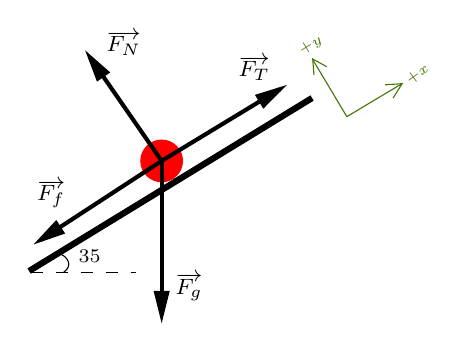
\begin{tikzpicture}[x=0.75pt,y=0.75pt,yscale=-1,xscale=1]
	%uncomment if require: \path (0,300); %set diagram left start at 0, and has height of 300

	%Shape: Ellipse [id:dp4017134135670819] 
	\draw  [color={rgb, 255:red, 255; green, 0; blue, 0 }  ,draw opacity=1 ][fill={rgb, 255:red, 255; green, 0; blue, 0 }  ,fill opacity=1 ] (111.34,112.66) .. controls (111.34,107.12) and (115.83,102.64) .. (121.37,102.64) .. controls (126.9,102.64) and (131.39,107.12) .. (131.39,112.66) .. controls (131.39,118.2) and (126.9,122.69) .. (121.37,122.69) .. controls (115.83,122.69) and (111.34,118.2) .. (111.34,112.66) -- cycle ;
	%Straight Lines [id:da11049691654941651] 
	\draw [line width=1.5]    (121.37,112.66) -- (86.79,62.71) ;
	\draw [shift={(84.51,59.43)}, rotate = 55.3] [fill={rgb, 255:red, 0; green, 0; blue, 0 }  ][line width=0.08]  [draw opacity=0] (15.6,-3.9) -- (0,0) -- (15.6,3.9) -- cycle    ;
	%Straight Lines [id:da9494684383086442] 
	\draw [line width=1.5]    (121.37,112.66) -- (121.37,186.86) ;
	\draw [shift={(121.37,190.86)}, rotate = 270] [fill={rgb, 255:red, 0; green, 0; blue, 0 }  ][line width=0.08]  [draw opacity=0] (15.6,-3.9) -- (0,0) -- (15.6,3.9) -- cycle    ;
	%Shape: Right Angle [id:dp18042975486392487] 
	\draw  [color={rgb, 255:red, 65; green, 117; blue, 5 }  ,draw opacity=1 ] (193.86,63.38) -- (210.59,91.34) -- (237.26,75.37) ;
	\draw  [color={rgb, 255:red, 65; green, 117; blue, 5 }  ,draw opacity=1 ] (229.05,75.99) -- (237.23,75.45) -- (232.86,82.39) ;
	\draw  [color={rgb, 255:red, 65; green, 117; blue, 5 }  ,draw opacity=1 ] (194.75,71.23) -- (194.15,63.58) -- (200.91,67.29) ;

	%Shape: Rectangle [id:dp3435108917878682] 
	\draw  [fill={rgb, 255:red, 0; green, 0; blue, 0 }  ,fill opacity=1 ] (58.37,166.64) -- (194.25,83.57) -- (192.96,81.45) -- (57.08,164.53) -- cycle ;
	%Straight Lines [id:da04201278790866225] 
	\draw [line width=1.5]    (121.37,112.66) -- (178.24,78.16) ;
	\draw [shift={(181.66,76.09)}, rotate = 148.76] [fill={rgb, 255:red, 0; green, 0; blue, 0 }  ][line width=0.08]  [draw opacity=0] (15.6,-3.9) -- (0,0) -- (15.6,3.9) -- cycle    ;
	%Straight Lines [id:da3784033887963598] 
	\draw [line width=1.5]    (121.37,112.66) -- (63.01,150.72) ;
	\draw [shift={(59.66,152.91)}, rotate = 326.89] [fill={rgb, 255:red, 0; green, 0; blue, 0 }  ][line width=0.08]  [draw opacity=0] (15.6,-3.9) -- (0,0) -- (15.6,3.9) -- cycle    ;
	%Curve Lines [id:da8374647738641394] 
	\draw    (74.27,166.2) .. controls (78.86,163.07) and (75.76,158.84) .. (72.93,157.71) ;
	%Straight Lines [id:da35140741666861075] 
	\draw  [dash pattern={on 4.5pt off 4.5pt}]  (58.37,166.64) -- (108.8,166.64) ;

	% Text Node
	\draw (93.59,48.74) node [anchor=north west][inner sep=0.75pt]  [font=\footnotesize] [align=left] {$\displaystyle \overrightarrow{F_{N}}$};
	% Text Node
	\draw (126.77,165.7) node [anchor=north west][inner sep=0.75pt]  [font=\footnotesize] [align=left] {$\displaystyle \overrightarrow{F_{g}}$};
	% Text Node
	\draw (236.41,72) node [anchor=north west][inner sep=0.75pt]  [font=\tiny,color={rgb, 255:red, 65; green, 117; blue, 5 }  ,opacity=1 ,rotate=-323.81] [align=left] {$\displaystyle +x$};
	% Text Node
	\draw (184.88,57.25) node [anchor=north west][inner sep=0.75pt]  [font=\tiny,color={rgb, 255:red, 65; green, 117; blue, 5 }  ,opacity=1 ,rotate=-328.27] [align=left] {$\displaystyle +y$};
	% Text Node
	\draw (157.19,60.68) node [anchor=north west][inner sep=0.75pt]  [font=\footnotesize] [align=left] {$\displaystyle \overrightarrow{F_{T}}$};
	% Text Node
	\draw (60.09,120.55) node [anchor=north west][inner sep=0.75pt]  [font=\footnotesize] [align=left] {$\displaystyle \overrightarrow{F_{f}}$};
	% Text Node
	\draw (80.04,154.12) node [anchor=north west][inner sep=0.75pt]  [font=\scriptsize] [align=left] {$\displaystyle 35\degree $};


\end{tikzpicture}
\end{minipage}%
\begin{minipage}[t]{.5\textwidth}
	\underline{$m_{2}$ FBD:}
	\tikzset{every picture/.style={line width=0.75pt}} %set default line width to 0.75pt        

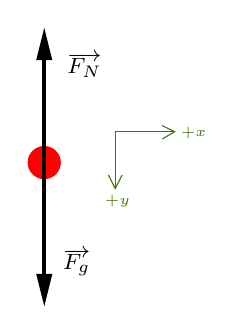
\begin{tikzpicture}[x=0.75pt,y=0.75pt,yscale=-1,xscale=1]
	%uncomment if require: \path (0,300); %set diagram left start at 0, and has height of 300

	%Shape: Ellipse [id:dp9950989906592862] 
	\draw  [color={rgb, 255:red, 255; green, 0; blue, 0 }  ,draw opacity=1 ][fill={rgb, 255:red, 255; green, 0; blue, 0 }  ,fill opacity=1 ] (182.07,109.96) .. controls (182.07,105.7) and (185.53,102.25) .. (189.79,102.25) .. controls (194.05,102.25) and (197.5,105.7) .. (197.5,109.96) .. controls (197.5,114.22) and (194.05,117.68) .. (189.79,117.68) .. controls (185.53,117.68) and (182.07,114.22) .. (182.07,109.96) -- cycle ;
	%Straight Lines [id:da5274227465782517] 
	\draw [line width=1.5]    (189.79,109.96) -- (189.79,49.02) ;
	\draw [shift={(189.79,45.02)}, rotate = 90] [fill={rgb, 255:red, 0; green, 0; blue, 0 }  ][line width=0.08]  [draw opacity=0] (15.6,-3.9) -- (0,0) -- (15.6,3.9) -- cycle    ;
	%Straight Lines [id:da9183971803471973] 
	\draw [line width=1.5]    (189.79,109.96) -- (189.79,175.19) ;
	\draw [shift={(189.79,179.19)}, rotate = 270] [fill={rgb, 255:red, 0; green, 0; blue, 0 }  ][line width=0.08]  [draw opacity=0] (15.6,-3.9) -- (0,0) -- (15.6,3.9) -- cycle    ;
	%Shape: Right Angle [id:dp316002013024695] 
	\draw  [color={rgb, 255:red, 65; green, 117; blue, 5 }  ,draw opacity=1 ] (252.86,94.98) -- (224.03,94.98) -- (224.03,122.5) ;
	\draw  [color={rgb, 255:red, 65; green, 117; blue, 5 }  ,draw opacity=1 ] (227.29,115.98) -- (223.98,122.44) -- (220.7,115.97) ;
	\draw  [color={rgb, 255:red, 65; green, 117; blue, 5 }  ,draw opacity=1 ] (246.5,92.09) -- (252.58,95.12) -- (246.69,98.56) ;


	% Text Node
	\draw (199.67,55.84) node [anchor=north west][inner sep=0.75pt]  [font=\footnotesize] [align=left] {$\displaystyle \overrightarrow{F_{N}}$};
	% Text Node
	\draw (197.63,150.28) node [anchor=north west][inner sep=0.75pt]  [font=\footnotesize] [align=left] {$\displaystyle \overrightarrow{F_{g}}$};
	% Text Node
	\draw (254.44,91.67) node [anchor=north west][inner sep=0.75pt]  [font=\tiny,color={rgb, 255:red, 65; green, 117; blue, 5 }  ,opacity=1 ] [align=left] {$\displaystyle +x$};
	% Text Node
	\draw (217.88,124.61) node [anchor=north west][inner sep=0.75pt]  [font=\tiny,color={rgb, 255:red, 65; green, 117; blue, 5 }  ,opacity=1 ] [align=left] {$\displaystyle +y$};


\end{tikzpicture}
\end{minipage}
\\Since there is constant speed, $\vec{F_{net_{x}}}=0$\\
\newline
\begin{minipage}[t]{0.3\textwidth}
	\underline{$m_{1}$:}
	\begin{flalign*}
		\vec{F_{net_{x}}} & = \vec{F_{T}} - \vec{F_{f}}  - \vec{F_{g_{x}}}          \\
		0                 & = \vec{F_{T}} - \vec{F_{f}} - 0.45(9.81)\sin35\degree   \\
		\vec{F_{T}}       & = \vec{F_{f}} + 0.45(9.81)\sin35\degree                 \\
		\vec{F_{T}}       & = \vec{F_{f}}+2.53~\text{N[uphill]}                   &
	\end{flalign*}
\end{minipage}%
\hspace{0.5cm}
\begin{minipage}[t]{0.3\textwidth}
	\underline{$m_{2}$:}
	\begin{flalign*}
		\vec{F_{net_{y}}} & = \vec{F_{g}}-\vec{F_{T}}          \\
		0                 & = 0.35 \times 9.81 - \vec{F_{T}}   \\
		\vec{F_{T}}       & = 3.43~\text{N[up]}              &
	\end{flalign*}
\end{minipage}%
\hspace{0.2cm}
\begin{minipage}[t]{0.3\textwidth}
	\underline{Set Equations for}\\
	\underline{$F_{T}$ Equal:}
	\begin{flalign*}
		3.43        & = \vec{F_{f}}+2.53         \\
		\vec{F_{f}} & = 0.9~\text{N[downhill]} &
	\end{flalign*}
\end{minipage}%
\vspace{4mm}
\begin{minipage}[t]{0.5\textwidth}
	\underline{Solve for Friction Coefficient:}
	\begin{flalign*}
		\vec{F_{f}} & = \mu_{f}\vec{F_{N}}                   & \\
		0.9         & = \mu_{f}\times0.45(9.81)\cos35\degree   \\
		\mu_{f}     & = \frac{0.9}{0.45(9.81)\cos35\degree}    \\
		\mu_{f}     & = 0.249                                  \\
		\mu_{f}     & = 0.25
	\end{flalign*}
\end{minipage}\\
\\\framebox{$\therefore$ The coefficient of friction between the box and incline is \textbf{0.25}.}
\end{document}